\documentclass{BeamerTemplate}

\title{Module 4 - Covariance et corrélation}

\date{\today}

\begin{document}
\begin{frame}[t]
  \titlepage
\end{frame}

%-------------------------------------------------------------------------------------------------------------------------------------





%%%%%%%%%%%%%%%%%%%%%%%%%%%%%%%%%%%
%%%%%%%%%%%%%%%%%%%%%%%%%%%%%%%%%%%
%%%%%%%%%%%%%%%%%%%%%%%%%%%%%%%%%%%



\section{Distributions conjointes}

\subsection{Théorie générale}

\begin{frame}[t]{Une expérience, plusieurs variables d'intérêt}

{\small
On peut être intéressés \alert{simultanément} par la valeur de plusieurs variables aléatoires.

\medskip
\underline{\bf Exemple:} Le réservoir d'un barrage est alimenté par 2 rivières. Soit
$X_i$= le volume d'eau déversé dans le réservoir par la rivière $i$ en une journée
($i=1,2$).
\medskip

%La compagnie qui gère ce barrage est intéressée par le compor\-te\-ment conjoint des 4 variables,  puisque
Le niveau d'eau dans le réservoir dépend du volume d'eau apporté par les 2 rivières, et ces volumes ne sont \alert{pas indépendants} les uns des autres.
\medskip

On voudra déterminer la \alert{loi conjointe du vecteur aléatoire ${\boldsymbol{X}}=(X_1, X_2)$}.
}



\end{frame}

\begin{frame}[t]
 \frametitle{Besoin de modèles conjoints}
 Quand les variables formant un vecteur aléatoire évoluent de manière indépendante, on peut utiliser la théorie précédente pour calculer des probabilités, moyennes, variances, etc.

 \bigskip
 Quand la valeur d'une variable contient de l'information sur la distribution des autres variables, on doit \alert{étudier les probabilités
 de façon conjointe}.

 \vspace{2cm}


\end{frame}


\begin{frame}[t]{Densité conjointe à 2 dimensions}
\begin{center}
    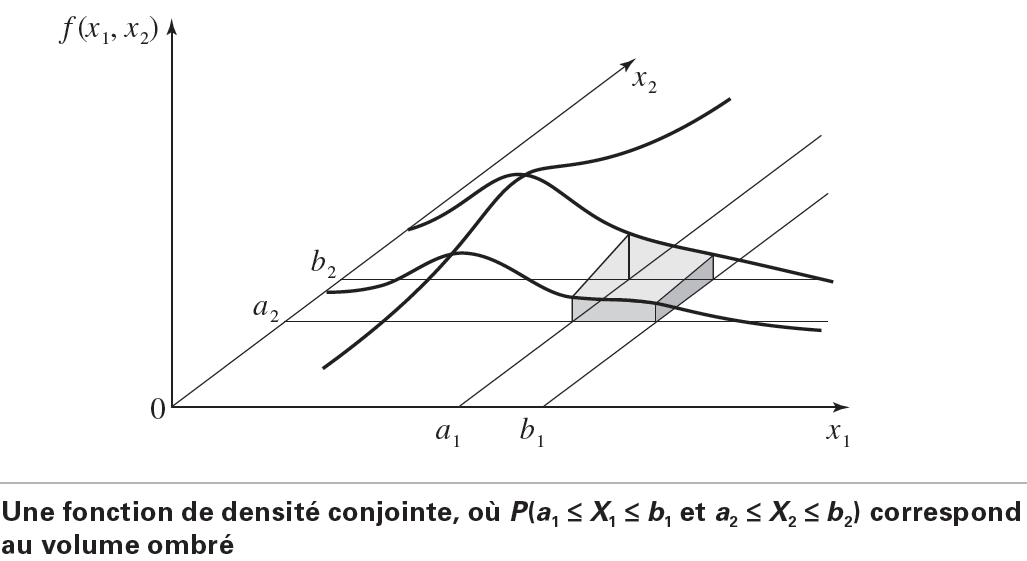
\includegraphics[width=9.5cm]{Images/Module 4/Fig3-4.PNG}

\end{center}

\end{frame}

\begin{frame}[t]{Densité conjointe à 2 dimensions}
Dans ce cours, nous ne ferons aucun calcul à partir de densités conjointes.

\bigskip

Nous nous intéresserons seulement au lien linéaire entre deux variables aléatoires.

\bigskip

Nous introduirons la covariance et la corrélation.
    
\end{frame}

\section{Covariance et corrélation}



\begin{frame}[t]
 \frametitle{Covariance entre deux variables}

 {\small
 Soit $X$ et $Y$ deux variables aléatoires. 
 On peut mesurer leur association linéaire.
\begin{Boite}{Covariance}
Soit deux variables $X$ et $Y$ d'espérances respectives $\mu_X$ et $\mu_Y$.\\
La \alert{covariance} entre $X$ et $Y$ est définie par
$$
Cov(X,Y)=E[(X-\mu_X)(Y-\mu_Y)].
$$
\end{Boite}
\uncover<2->{
Covariance = indicateur de la \alert{force du lien linéaire} qui unit deux variables.\\

Le signe de la covariance (+ ou -) nous dit si les variables ont tendance à prendre
de fortes valeurs par rapport à leur moyenne en même temps ou non.}

\medskip

\uncover<3->{\alert{Attention:} $X\perp Y \rightarrow Cov(X,Y)=0$, mais $Cov(X,Y)=0 \notrightarrow X\perp Y$}
}


\end{frame}

\begin{frame}[t]
\frametitle{Interprétation de la covariance}

{\renewcommand{\baselinestretch}{0.9}
\begin{tabular}{|p{3.3cm}|p{3.3cm}|p{6cm}|}\hline
\alert{Cov. positive} & \alert{Cov. négative} & \alert{Covariance nulle}\\\hline
{\footnotesize $X$ et $Y$ prennent de fortes ou faibles valeurs par rapport à leur moyenne en même temps}&
{\footnotesize $X$ prend de fortes valeurs quand $Y$ en prend de faibles par rapport à leur moyenne et vice versa}&
{\footnotesize Pas de tendance linéaire dominante.}\\
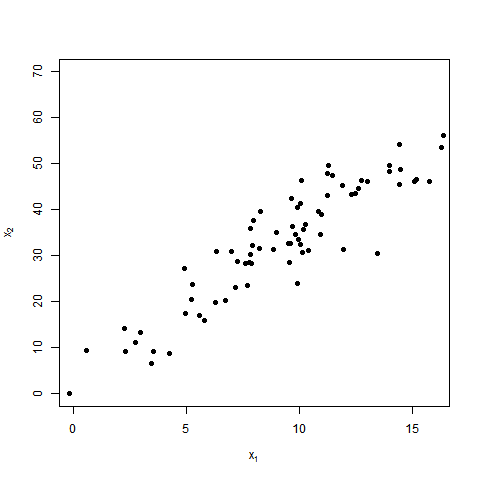
\includegraphics[width=3cm]{Images/Module 4/cov-pos.png}&
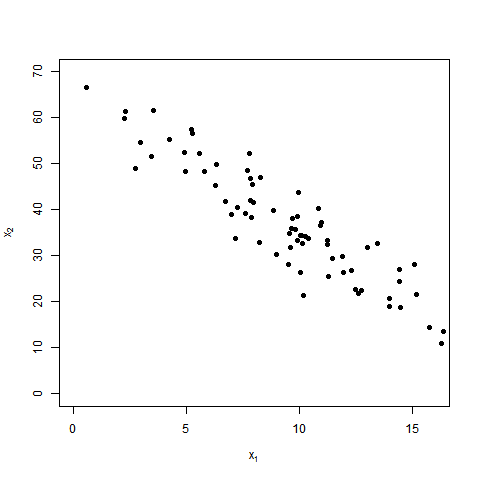
\includegraphics[width=3cm]{Images/Module 4/cov-neg.png}&
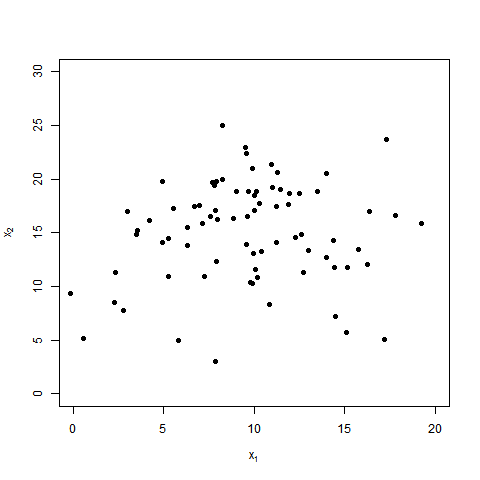
\includegraphics[width=2.9cm]{Images/Module 4/cov-indep.png}
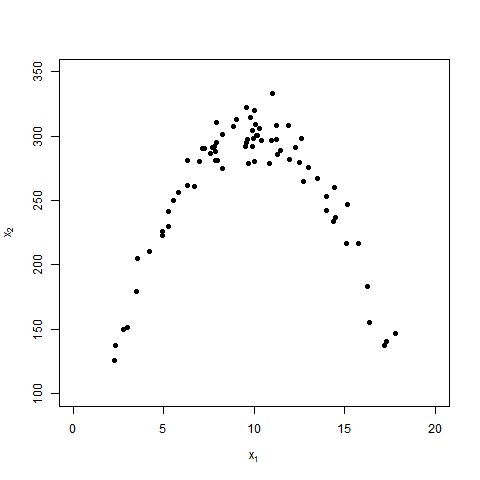
\includegraphics[width=2.9cm]{Images/Module 4/cov-para.png}\\\hline
\end{tabular}
\medskip

}


\end{frame}

\begin{frame}[t]
 \frametitle{Propriétés de la covariance}
 \begin{itemize}\itemsep4mm
% \item $Cov(a, X)=$
 \item $Cov(X, X)=V(X)$
 \item $Cov(aX, bY)=abCov(X, Y)$
 \item $Cov(X+c, Y+d)=Cov(X, Y)$
 \item $V(X+Y)=V(X)+V(Y)+2 Cov(X,Y)$
 \item $V(X-Y)=V(X)+V(Y)-2 Cov(X,Y)$
\item $V(aX+bY)=a^2V(X)+b^2V(Y)+2abCov(X,Y)$
\item {\small $V(a_0+a_1X_1+\cdots+a_kX_k)=
{\color{blue}{ a_1^2\sigma^2_1+\cdots+a_k^2\sigma^2_k}}
+2\sum\limits_{i<i'}\sum%\limits_{i'=1}^k
a_ia_{i'}Cov(X_i,X_{i'})$}
\end{itemize}
\end{frame}

\begin{frame}[t]{ }

\centerline{\LARGE\bf \alert{QUIZ !}}
\bigskip
\begin{itemize}\itemsep1.5cm
\item  Que peut-on dire de $Cov(5,\, X)$? % 0
\item Vrai ou Faux: $Cov(X,\,3Y)=Cov(Y,\,3X)$? % Vrai
\item Si $X$ est mesuré en $^\circ C$ et $Y$ en secondes, quelles sont les unités de la covariance?
\end{itemize}


\end{frame}

\begin{frame}[t]
 \frametitle{Corrélation}

{\small
Soit les variables aléatoires $W, X, Y$ et $Z$. Nous ne pouvons pas directement comparer $Cov(W,X)$ et $Cov(Y,Z)$ pour savoir quelle paire de variables a la plus forte association linéaire, parce que la covariance dépend de l'échelle des variables.\\


%le coefficient de corrélation.
\begin{Boite}{Coefficient de corrélation}
Soit deux variables $X$ et $Y$ de variances respectives $\sigma^2_X$ et $\sigma^2_Y$.\\
Le \alert{coefficient de corrélation} entre $X$ et $Y$ est défini par
$$
\rho_{X,Y}=corr(X,Y)=\frac{Cov(X,Y)}{\sqrt{\sigma^2_X\;\sigma^2_Y}}.
$$
\end{Boite}

Plus les valeurs de $X$ et $Y$ sont fortement corrélées, plus la valeur
de $\rho_{X,Y}$ sera proche de $-1$ ou $1$.


Pour alléger l'écriture, si seulement deux variables sont présentes, on écrit $\rho$.
}
\end{frame}

\begin{frame}[t]{Quelques valeurs de corrélations}

{\small Voici quelques nuages de points échantillonnés à partir de distributions conjointes ayant les corrélations théoriques précisées.}
\begin{center}
    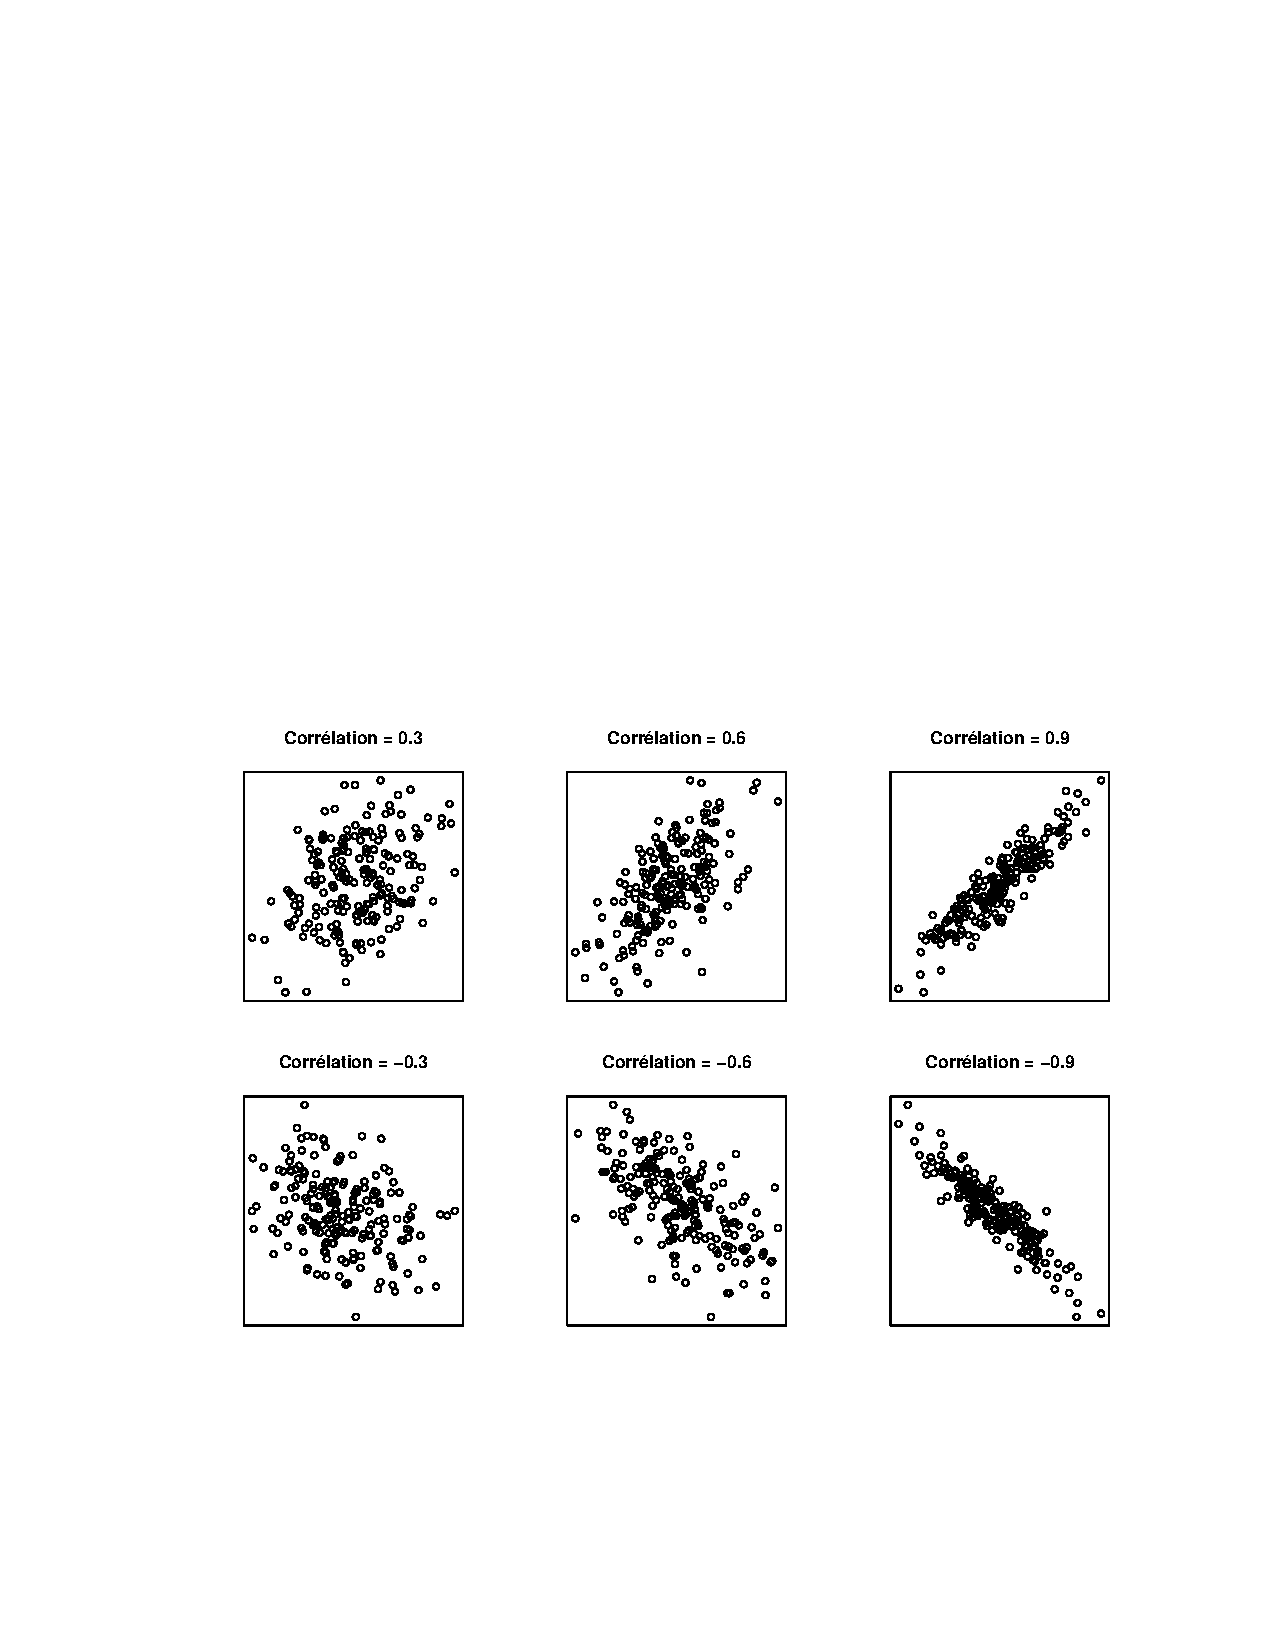
\includegraphics[scale = 0.58]{Images/Module 4/correlations.pdf}
\end{center}

 \end{frame}

\begin{frame}[t]{}

\centerline{\LARGE\bf \alert{QUIZ !}}
\bigskip
{\small Sauriez-vous tracer un nuage de points pour lequel...}

\begin{itemize}\itemsep2cm
\item  $\rho_{X,Y}=0$?
\item $\rho_{X,Y}=-1$?
\end{itemize}
\vspace{1.5cm}


 \end{frame}

\begin{frame}[t]
 \frametitle{Exemple 1}

{\small
Soit $X$, $Y$ et $W$ trois variables avec
\begin{itemize}
\item $E(X)=1$, $E(Y)=0$, $E(W)=0$
\item $V(X)=16$, $V(Y)=4$, $V(W)=25$
\item $Cov(X,Y)=-2$, et $W$ est indépendante de $X$ et de $Y$.
\end{itemize}
Calculez les quantités suivantes.

\begin{enumerate}[(i)]\itemsep 9mm
\item $E(3+4X-Y+W)$
\end{enumerate}
}
%{\tiny (Plus d'espace à la p. suivante ...)}
\end{frame}

\begin{frame}[t]
 \frametitle{Exemple 1 (suite)}

\begin{enumerate}[(i)]\itemsep 3cm
\item[(ii)] $V(3+4X-Y+W)$
\item[(iii)] $corr(X,Y)$.
\end{enumerate}

{\ }
\end{frame}

%Pour (i), on utilise la formule (\ref{eq:ecorr}) qui nous dit que
%$E(3+4X-Y+W)=3+4E(X)+(-1)E(Y)+(1)E(W)=3+(4)(1)+(-1)(0)+(1)(0)=7$. Pour (ii),
%il faut prendre la formule (\ref{eq:vcorr}) qui nous dit que
%$V(3+4X-Y+W)=(4)^2V(X)+(-1)^2V(Y)+(1)^2V(W)+2(4)(-1)Cov(X,Y)+2(4)(1)Cov(X,W)
%+2(-1)(1)Cov(Y,W)=(4)^2(16)+(-1)^2(4)+(1)^2(25)+2(4)(-1)(-2)+2(4)(1)(0)
%+2(-1)(1)(0)=301$. Finalement pour (iii) on doit utiliser la définition donnée par
%l'équation (\ref{eq:corr}), donc $\rho_{X,Y}=Cov(X,Y)/\sqrt{V(X)V(Y)}=-2/\sqrt{(16)(4)}=-0.25.$
%\end{exemple}


\begin{frame}[t]{Réponses aux exemples}

{\scriptsize
\begin{enumerate}
  \item
        \begin{enumerate}[(i)]
        \item $E(3+4X-Y+W)=7$
        \item$V(3+4X-Y+W)=301$
        \item $corr(X,Y)=-0.25$.
        \end{enumerate}


 \end{enumerate}
 }
\end{frame}


\end{document}